\section{Funciones diferenciales}

Sea $f : D \subset \mathbb{R}^2 \to \mathbb{R}$ y $A = (x_0, y_0) \in D^\circ$. Se dice que $f$ es diferenciable
en $A$ si se cumple:

\[
\lim_{(x,y) \to (x_0,y_0)}
\frac{f(x, y) - \bigl(f(x_0, y_0) + \tfrac{\partial f}{\partial x}(x_0, y_0)(x - x_0) + \tfrac{\partial f}{\partial y}(x_0, y_0)(y - y_0)\bigr)}
{\sqrt{(x - x_0)^2 + (y - y_0)^2}} = 0.
\]


\begin{figure}
    \centering
    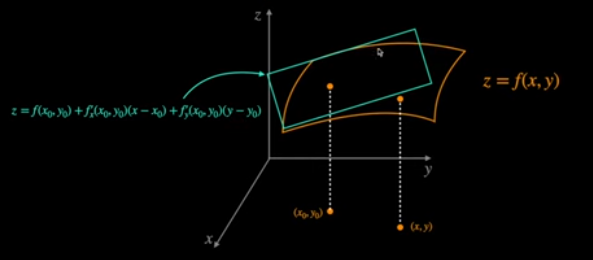
\includegraphics[width=0.5\textwidth]{img/plano.png}
    \caption{El numerador tiende a cero más rápido que el denominador.}
    \label{}
\end{figure}

\subsection{Teoremas}
\begin{enumerate}
    \item Si $f:D \subset \mathbb{R}^n \to \mathbb{R}^m$, es diferenciable en $A$ entonces $f$
    es continua en $A$. Si $f$ no es continua en $A$ entonces no es diferenciable en $A$.
    \item Si $f:D \subset \mathbb{R}^n \to \mathbb{R}^m$, es diferenciable en $A$ entonces $f$
    es derivable en toda dirección en $A$, es decir, $\forall \check{r} \in \mathbb{R}$ existe
    $f'(A, \check{r})$
    \item Si $f:D \subset \mathbb{R}^n \to \mathbb{R}^m$, $f \in C^1 (E(A))$ entonces $f$ es diferenciable en $A$.
\end{enumerate} 

\begin{figure}[H]
    \centering
    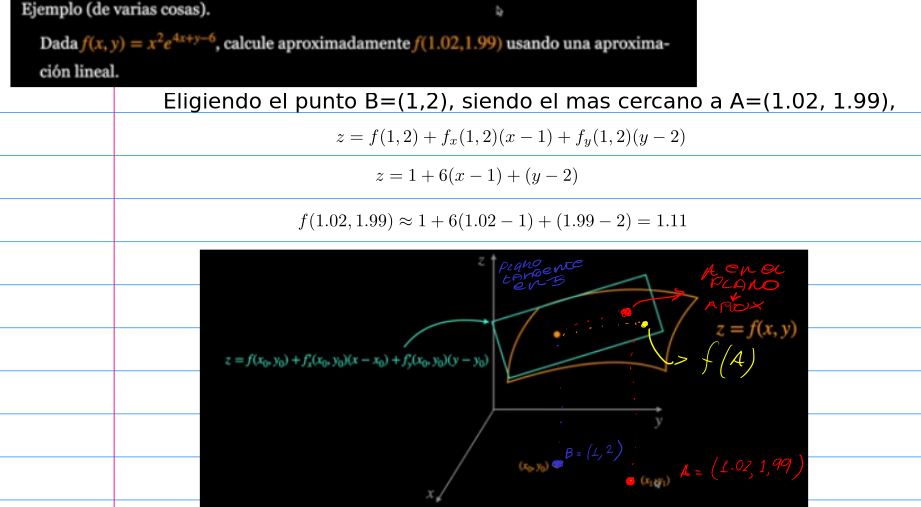
\includegraphics[width=0.8\textwidth]{img/ej-dif.png}
    \label{}
\end{figure}


\subsection{Gradientes y derivadas direccionales}

Sea $\check{r}=(a,b)$, las derivadas direccionales de una función lineal de dos variables:
$$
f'((x_0, y_0), \check{r}) = 
\frac{\partial f}{\partial x} (x_0, y_0) a
+
\frac{\partial f}{\partial y} (x_0, y_0) b
$$
\subsection*{Definición}
Si $f:D \subset \mathbb{R}^2 \to \mathbb{R}$ es diferenciable en $A=(x_0, y_0)$,
el vector $(\frac{\partial f}{\partial x} (x_0, y_0), \frac{\partial f}{\partial y} (x_0, y_0))$
se llama \textbf{gradiente} de $f$ en $A$ y se denota por:

$$\nabla f (x_0, y_0) =
(\frac{\partial f}{\partial x} (x_0, y_0), \frac{\partial f}{\partial y} (x_0, y_0))
$$

$$
f'((x_0, y_0), \check{r}) = 
\nabla f (x_0, y_0) \cdot \check{r}
$$

\subsection*{Propiedades}
Si $f:D \subset \mathbb{R}^2 \to \mathbb{R}$ es diferenciable en $A=(x_0, y_0)$,
entonces:

$$
f'((x_0, y_0), \check{r}) = 
\nabla f (x_0, y_0) \cdot \check{r}
$$
Y dado a que es un producto interno entre dos vectores, se cumple que:
$$
f'((x_0, y_0), \check{r}) =
||\nabla f (x_0, y_0)|| \cdot ||\check{r}|| \cdot \cos \theta
$$
Donde $\theta$ es el ángulo entre los vectores $\nabla f (x_0, y_0)$ y $\check{r}$.
Y como $||\check{r}|| = 1$, y $-1 \leq \cos \theta \leq 1$, se cumple que:

$$
-||\nabla f (x_0, y_0)|| \leq f'((x_0, y_0), \check{r}) \leq ||\nabla f (x_0, y_0)||
$$ 


\begin{itemize}
    \item La máxima derivada direccional se da con $||\nabla f (x_0, y_0)||$ y se alcanza con la dirección 
    $\check{r}_{max} = \frac{\nabla f (x_0, y_0)}{||\nabla f (x_0, y_0)||}$.
    \item La mínima derivada direccional se da con $-||\nabla f (x_0, y_0)||$ y se alcanza con la dirección 
    $\check{r}_{min} = -\frac{\nabla f (x_0, y_0)}{||\nabla f (x_0, y_0)||}$.
    \item Se obtienen derivadas direccionales nulas cuando $\check{r} \perp \nabla f (x_0, y_0)$.
\end{itemize}